%%%%%%%%%%%%%%%%%%%%%%%%%%%%%%%%%%%%%%%%%
% Beamer Presentation
% LaTeX Template
% Version 2.0 (27/IX/15)
%
% This template has been downloaded from http://www.LaTeXTemplates.com
% and modified by Semen Martynov <semen.martynov@gmail.com>
%
% License:
% CC BY-NC-SA 3.0 (http://creativecommons.org/licenses/by-nc-sa/3.0/)
%
%%%%%%%%%%%%%%%%%%%%%%%%%%%%%%%%%%%%%%%%%

%----------------------------------------------------------------------------------------
%	PACKAGES AND THEMES
%----------------------------------------------------------------------------------------

\documentclass{beamer}

\mode<presentation> {

% The Beamer class comes with a number of default slide themes
% which change the colors and layouts of slides. Below this is a list
% of all the themes, uncomment each in turn to see what they look like.

%\usetheme{default}
%\usetheme{AnnArbor}
%\usetheme{Antibes}
%\usetheme{Bergen}
%\usetheme{Berkeley}
%\usetheme{Berlin}
%\usetheme{Boadilla}
%\usetheme{CambridgeUS}
%\usetheme{Copenhagen}
%\usetheme{Darmstadt}
%\usetheme{Dresden}
%\usetheme{Frankfurt}
%\usetheme{Goettingen}
%\usetheme{Hannover}
%\usetheme{Ilmenau}
%\usetheme{JuanLesPins}
%\usetheme{Luebeck}
\usetheme{Madrid}
%\usetheme{Malmoe}
%\usetheme{Marburg}
%\usetheme{Montpellier}
%\usetheme{PaloAlto}
%\usetheme{Pittsburgh}
%\usetheme{Rochester}
%\usetheme{Singapore}
%\usetheme{Szeged}
%\usetheme{Warsaw}

% As well as themes, the Beamer class has a number of color themes
% for any slide theme. Uncomment each of these in turn to see how it
% changes the colors of your current slide theme.

%\usecolortheme{albatross}
%\usecolortheme{beaver}
%\usecolortheme{beetle}
%\usecolortheme{crane}
%\usecolortheme{dolphin}
%\usecolortheme{dove}
%\usecolortheme{fly}
%\usecolortheme{lily}
%\usecolortheme{orchid}
%\usecolortheme{rose}
%\usecolortheme{seagull}
%\usecolortheme{seahorse}
%\usecolortheme{whale}
%\usecolortheme{wolverine}

%\setbeamertemplate{footline} % To remove the footer line in all slides uncomment this line
%\setbeamertemplate{footline}[page number] % To replace the footer line in all slides with a simple slide count uncomment this line

%\setbeamertemplate{navigation symbols}{} % To remove the navigation symbols from the bottom of all slides uncomment this line
\setbeamertemplate{caption}[numbered] % Image numbers
}

%%%% Charset (don't forget about texlive-lang-cyrillic)
\usepackage{cmap}							% make PDF files searchable and copyable
\usepackage[utf8x]{inputenc}				% accept different input encodings
\usepackage[T2A]{fontenc}					% russian font
\usepackage[russian]{babel}					% multilingual support (T2A)

%%%% Graphics
%\usepackage[dvipsnames]{xcolor}			% driver-independent color extensions
\usepackage{graphicx}						% enhanced support for graphics
\usepackage{wrapfig}						% produces figures which text can flow around

%%%% Math
\usepackage{amsmath}						% American Mathematical Society (AMS) math facilities
\usepackage{amsfonts}						% fonts from the AMS
\usepackage{amssymb}						% additional math symbols

%%%% Typograpy (don't forget about cm-super)
\usepackage{microtype}						% subliminal refinements towards typographical perfection
%\linespread{1.3}							% line spacing
\setlength{\parindent}{0pt}					% we don't want any paragraph indentation
\usepackage{parskip}						% some distance between paragraphs

%%%% Tables
\usepackage{booktabs}						% Allows the use of \toprule, \midrule and \bottomrule in tables
%\usepackage{tabularx}						% tables with variable width columns
%\usepackage{multirow}						% for tabularx
%\usepackage{hhline}							% for tabularx

%%%% Graph
%\usepackage{tikz}							% package for creating graphics programmatically
%\usetikzlibrary{arrows}						% edges for tikz

%%%% Other
%\usepackage{url}							% verbatim with URL-sensitive line breaks
%\usepackage{fancyvrb}						% sophisticated verbatim text (with box)

\makeatletter
\def\verbatim{\tiny\@verbatim \frenchspacing\@vobeyspaces \@xverbatim}
\makeatother

%----------------------------------------------------------------------------------------
%	TITLE PAGE
%----------------------------------------------------------------------------------------

\title[Динамический анализ приложений]{Введение в динамический анализ приложений на примере Intel Pin} % The short title appears at the bottom of every slide, the full title is only on the title page

\author{Чёрная команда} % Your name
\institute[СПбПУ] % Your institution as it will appear on the bottom of every slide, may be shorthand to save space
{
Санкт-Петербургский политехнический университет Петра Великого \\ % Your institution for the title page
\medskip
\textit{Антон Абрамов <abramov91@mail.ru>\\
Владислав Бусаров <happyfanik@yandex.ru>\\
Сергей Дедков <dsv.mail@yandex.ru>\\
Семён Мартынов <semen.martynov@gmail.com>\\
Николай Патраков <noon.vlg@gmail.com>} % Your email address
}
\date{\today} % Date, can be changed to a custom date

\begin{document}

\begin{frame}
\titlepage % Print the title page as the first slide
\end{frame}

\begin{frame}
\frametitle{Содержание} % Table of contents slide, comment this block out to remove it
\tableofcontents % Throughout your presentation, if you choose to use \section{} and \subsection{} commands, these will automatically be printed on this slide as an overview of your presentation
\end{frame}

%----------------------------------------------------------------------------------------
%	PRESENTATION SLIDES
%----------------------------------------------------------------------------------------

%------------------------------------------------
\section{Введение}
%------------------------------------------------

\begin{frame}
\frametitle{Введение: динамический анализ}
Анализ программы -- это один из фундаментальных этапов процесса разработки ПО. Он включает анализ с целью выявления поведенческих особенностей программы в период выполнения. Принято говорить о двух типа анализа: статический (изучался в курсе Моисеева М.Ю.) и динамический.\\~\\

Преимуществом статического анализа является 100\% покрытие кода, преимущество динамического анализа в том, что он может давать детализированную и точную информацию. Существует множество способов профилирования программы, например использование событий инфраструктуры, точки подключения к ОС и динамическое оснащение программы средствами мониторинга и протоколирования (instrumentation). Хотя Visual Studio или GDB предоставляет инфраструктуру профилирования, их возможности ограниченны. Для всех сценариев динамического оснащения, кроме простейших, требуется более совершенная инфраструктура, которую может предоставить Pin.
\end{frame}

%------------------------------------------------

\begin{frame}
\frametitle{Введение: Pin}
Pin -- это инфраструктура динамического оснащения на уровне двоичного кода (\textbf{d}ynamic \textbf{b}inary \textbf{i}nstrumentation framework), позволяющая создавать средства анализа программ, называемые Pintool для платформ Windows и Linux.
\begin{itemize}
\item \textit{Инфраструктура} (framework) -- это набор кода, на основе которого пишется программа
\item \textit{Оснащение} (instrumentation) -- процесс анализа программы добавлением и/или модификацией кода
\item Понятие \textit{двоичный} указывает, что добавляемый или модифицируемый код, представляет собой машинный код в двоичной форме
\item Понятие \textit{динамический} указывает, что процесс оснащения осуществляется в период выполнения, пока программа работает.
\end{itemize}
\end{frame}


%------------------------------------------------

\begin{frame}
\frametitle{Введение: принцип работы Pin}

\begin{figure}
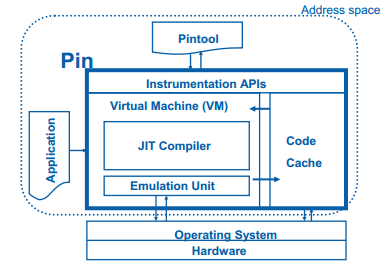
\includegraphics[scale=1]{302144}
\caption{Взаимодействие фреймворка и приложения}
\end{figure}

\end{frame}
%------------------------------------------------

\begin{frame}
\frametitle{Введение: основные возможности Pin}
Pin является закрытым ПО, но доступен для свободного скачивания и бесплатного использования для некоммерческих целей.\\~\\

В текущей версии (Pin 2.13) заявлена поддержка следующих платформ:
\begin{itemize}
\item Windows (IA32 и Intel64)
\item Linux (IA32 и Intel64)
\item Mac OS X (IA32 и Intel64)
\item Android (IA32)
\item Intel Xeon Phi (для суперкомпьютеров)
\end{itemize}
\end{frame}

%------------------------------------------------
\section{Установка}
%------------------------------------------------

\begin{frame}
\frametitle{Установка: инсталляция на основных системах}
\begin{block}{Системы на базе Arch Linux (из Arch User Repository)}
yaourt -Sy pin

\end{block}

\begin{block}{Системы на базе Debian/Ubuntu (из PPA)}
sudo add-apt-repository ppa:md+lp/pintool \&\& sudo apt-get update\\
sudo apt-get install -y pintool
\end{block}

\begin{block}{Системы на базе RHEL/Fedora}
sudo yum install -y pintool
\end{block}

\begin{block}{Системы семейства Windows (не рекомендуется)}
Бинарные файлы скачиваются с официального сайта Intel \url{http://intel.ly/1ysiBs4}
\end{block}
\end{frame}

%------------------------------------------------

\begin{frame}
\frametitle{Установка: проблемы}

\begin{block}{Ошибка}
При запуске на относительно свежем ядре (4+) программа завершалась со следующим сообщением\\
E: 4.1 is not a supported linux release:
\end{block}

\begin{block}{Решение}
Использование параметра \textit{-ifeellucky} позволяет использовать pin со свежими ядрами linux.
\end{block}

\begin{block}{Ошибка}
Не корректная работа с программами, откомпилированными свежей версией GCC (5+).
\end{block}

\begin{block}{Решение}
Использование параметра \textit{-fabi-version=2} позволяет использовать свежую версию ABI.
\end{block}

\end{frame}

%------------------------------------------------
\section{Pintool для трассировки операций чтения/записи}
%------------------------------------------------
\subsection{Гранулярность Pin}
%------------------------------------------------

\begin{frame}
\frametitle{Гранулярность Pin}
Оснащение программы -- вставка код в специфические места исследуемой программы (обычно непосредственно до или после выполнения конкретной инструкции или функции).\\~\\

Для выбора подходящего компромисса между производительностью и уровнем детализации, существует три основных уровня гранулярности для Pin:
\begin{itemize}
\item \textit{подпрограмма} (routine) -- может оказаться слишком общим
\item \textit{инструкция} (instruction) -- может приводить к катастрофическому падению производительности
\item \textit{образ} (image) -- требует символы
\end{itemize}

Помимо этого, существует \textit{трассировка}, которая помогает выполнять оснащение, не жертвуя производительностью или детализацией.
\end{frame}

%------------------------------------------------
\subsection{Исходный код}
%------------------------------------------------

\begin{frame}[fragile] % Need to use the fragile option when verbatim is used in the slide
\frametitle{Исходный код (1/3)}

\begin{block}{Вспомогательные функции}
\begin{verbatim}
#include <stdio.h> // стандартный заголовочный файл ввода-вывода
#include "pin.H" // задействовать Pin API

FILE * trace; // результат работы будут сохранены в журнал

// фиксация состояния регистра указателя инструкции и адреса памяти для операции ЧТЕНИЯ в журнал
VOID RecordMemRead(VOID * ip, VOID * addr) {
    fprintf(trace,"%p: R %p\n", ip, addr);
}

// фиксация состояния регистра указателя инструкции и адреса памяти для операции ЗАПИСИ в журнал
VOID RecordMemWrite(VOID * ip, VOID * addr) {
    fprintf(trace,"%p: W %p\n", ip, addr);
}

// процедура завершения вызываться при завершении оснащенной программы
VOID Fini(INT32 code, VOID *v) {
    fprintf(trace, "#eof\n");
    fclose(trace);
}

// вывод справочной информации
INT32 Usage() {
    PIN_ERROR( "This Pintool prints a trace of memory addresses\n" 
              + KNOB_BASE::StringKnobSummary() + "\n");
    return -1;
}
\end{verbatim}
\end{block}
\end{frame}

%------------------------------------------------

\begin{frame}[fragile] % Need to use the fragile option when verbatim is used in the slide
\frametitle{Исходный код (2/3)}

\begin{block}{Гранулярность на уровне инструкции -- функция Instruction()}
\begin{verbatim}
// Вызывается для каждой инструкции.
// Будем исследовать только те инструкции, которые читают или пишут в память.
VOID Instruction(INS ins, VOID *v) {

    //Операнды, гарантированно получающие управление
    UINT32 memOperands = INS_MemoryOperandCount(ins);

    // Итерируемся по всем операндам и инструкциям
    for (UINT32 memOp = 0; memOp < memOperands; memOp++)
    {
        // Для операций чтения:
        if (INS_MemoryOperandIsRead(ins, memOp))
        {
            INS_InsertPredicatedCall(
                ins, // Оснащаемая процедура
                IPOINT_BEFORE, //куда её вставлять (ПЕРЕД требуемой инструкцией)
                (AFUNPTR)RecordMemRead, //указатель на функцию анализа RecordMemRead
                IARG_INST_PTR, // аргументы, передаваемые в RecordMemRead
                IARG_MEMORYOP_EA, memOp, 
                IARG_END); // признак конца списка аргументов
        }
        // Для операций записи, аналогично
        if (INS_MemoryOperandIsWritten(ins, memOp))
        {
            INS_InsertPredicatedCall(
                ins, IPOINT_BEFORE, (AFUNPTR)RecordMemWrite, //указатель на функцию анализа RecordMemWrite
                IARG_INST_PTR, IARG_MEMORYOP_EA, memOp, IARG_END);
        }
    }
}
\end{verbatim}
\end{block}

\end{frame}

%------------------------------------------------

\begin{frame}[fragile] % Need to use the fragile option when verbatim is used in the slide
\frametitle{Исходный код (3/3)}
\begin{block}{Основная точка входа -- функция main()}
\begin{verbatim}
// Этот pintool генерирует трассировку всех адресов памяти, на которые ссылается программа
// (может быть полезно для отладки и для моделирования кэша данных в процессоре)
int main(int argc, char *argv[]) {

    // Разбор командной строки для инициализации переменных;
    // если переданы не верные параметры -- программа завершится
    if (PIN_Init(argc, argv)) return Usage();

    // Журнал работы будет называться pinatrace.out
    trace = fopen("pinatrace.out", "w");

    // Регистрируем функцию оснащения Instruction()
    INS_AddInstrumentFunction(Instruction, 0);
    // Регистрируем функцию завершения Fini()
    PIN_AddFiniFunction(Fini, 0);

    // Запуск анализируемой программы.
    // Эта функция никогда не возвращает управление функции main!!
    PIN_StartProgram();
    
    return 0;
}
\end{verbatim}
\end{block}
\end{frame}

%------------------------------------------------
\subsection{Запуск pintool}
%------------------------------------------------

\begin{frame}[fragile] % Need to use the fragile option when verbatim is used in the slide
\frametitle{Запуск pin}

Проведём исследование стандартной утилиты pwd

\begin{block}{Исследование системной утилиты pwd}
\begin{verbatim}
$ /opt/pin/intel64/bin/pinbin -t /opt/pin/source/tools/SimpleExamples/obj-intel64/pinatrace.so -- /bin/pwd
\end{verbatim}
\end{block}

Команда запуска состоит из трёх частей:
\begin{itemize}
\item /opt/pin/intel64/bin/pinbin путь к утилите pin
\item -t /opt/pin/source/tools/SimpleExamples/obj-intel64/pinatrace.so путь к рассмотренному ранее pintool (фактически представляет из себя динамическую библиотеку)
\item -{}- /bin/pwd путь к исследуемому бинарнику
\end{itemize}

\end{frame}
%------------------------------------------------

\begin{frame}[fragile] % Need to use the fragile option when verbatim is used in the slide
\frametitle{Результат запуска}
\begin{block}{Журнал исследования системной утилиты pwd\\ (последние 10 строк, общий объём порядка 3,5Мб)}
\begin{verbatim}
$ tail -n 25 pinatrace.out 
0x7f5c6717c178: W     0x7f5c674c3a40
0x7f5c6717c182: R     0x7f5c674c39e8
0x7f5c6717c196: R     0x7ffe8af72458
0x7f5c6717c197: R     0x7ffe8af72460
0x7f5c6717c198: R     0x7ffe8af72468
0x7f5c6717c19a: R     0x7ffe8af72470
0x7f5c6717c19c: R     0x7ffe8af72478
0x7f5c67138cda: W     0x7ffe8af72478
0x7f5c671c9fe3: R     0x7f5c674c2e68
#eof
\end{verbatim}
\end{block}

Каждая строка состоит из трёх полей
\begin{itemize}
\item Адрес инструментованной инструкции (IARG\_INST\_PTR), т.е. куда передано управление
\item Вид операции (чтение или запись)
\item Адрес операции (IARG\_MEMORYOP\_EA), т.е. эффективный адрес операции с памятью
\end{itemize}

\end{frame}

%------------------------------------------------
\section{Заключение}
%------------------------------------------------

\begin{frame}
\frametitle{Заключение}
Pin является эффективным инструментом для тонкого изучения работы программы.\\~\\

Основными достоинствами инструмента по нашему мнению является:
\begin{itemize}
\item Отсутствие необходимости изучать дополнительные языки -- для статического анализа требуется изучить Promela, для работы с GDB нужны знания Assembler, для работы с LLVM понимание синтаксиса IR
\item Возможность работать не имея исходных кодов -- достаточно частая необходимость, при изучении вредоносного ПО
\item Управляемая детализация отчётов - можно отфильтровать то, что требуется рассмотреть
\end{itemize}
\end{frame}

%------------------------------------------------
\section{Источники}
%------------------------------------------------

\begin{frame}
\frametitle{Источники}
\footnotesize{
\begin{thebibliography}{99} % Beamer does not support BibTeX so references must be inserted manually as below
\bibitem[Brays, 2014]{p1} Хади Браис
\newblock Инструментированные приложений: Анализ приложений с помощью Pin
\newblock \emph{MSDN Magazine Blog} - ноябрь, 2014.
\end{thebibliography}

\begin{thebibliography}{98}
\bibitem[Intel, 2015]{p1} Intel Corporation
\newblock Pin 2.13 User Guide
\newblock \emph{https://software.intel.com/sites/landingpage/pintool/docs/65163/Pin/html/index.html}
\end{thebibliography}
}
\end{frame}

%------------------------------------------------
\section{Вопросы}
%------------------------------------------------

\begin{frame}
\Huge{\centerline{Вопросы?}}
\end{frame}

%----------------------------------------------------------------------------------------

\end{document}